\documentclass[titlepage]{report}

\usepackage{titlesec}
\usepackage{lipsum}
\usepackage{graphicx}
\usepackage{wrapfig}

%setting for chapter font
\titleformat{\chapter}[display]
  {\Huge\bfseries}{}{1pt}{\Huge}
  
  
\author{ALL Author Names}
\title{\textbf{CustoNN2: Customizing Neural Networks on FPGAs}}  


\begin{document}

\maketitle

\tableofcontents
\newpage

\chapter{Introduction}
In recent times Convolutional Neural Networks (CNN) has gained immense popularity and is used in many applications such as Image classification , speech recognition etc. CNNs have become an industry standard and provide a near human accuracy. However CNN are computationally intensive models requiring large amount of processing power which calls for the need to have dedicated hardware for its acceleration. Graphics Processing Units (GPU) are conventionally used and provide satisfactory performance on some of the state-of-the-art CNN models. Although GPU provides good performance, its not flexible enough to accomodate multiple CNN models. One may need to re-design the entire GPU architecture for a particular CNN. This is where Field Programmable Gate Arrays (FPGA) proves to be much more beneficial in terms of flexibility and parallel processing. Some state-of the-art CNN models such as AlexNet , VGG16 and ResNet has shown considerable performance gain using FPGAs. Futhermore with the presence of various Software Development (SDK) Toolkit in the market such as Intel OpenVINO, Xilinx ML Suite and TVM has helped the developers to efficiently map their CNN models to the underlying architecture. Due to all of these factors CNN has become a popular choice for image classification applications.


\section{Why FPGA}
There are multiple hardware avaliable in the market such as CPU, GPU , ASIC and FPGA each used for a specific set of application. Among all of them FPGAs are becoming widely poplular and used in CNN based applications. Deep Neural Networks (DNN) benefit very much from using FPGA. DNN are math intensive models which execute the same or many mathematical operation. FPGAs have dedicated DSPs and ALUs to perform such Floating Point arithmetic operations. FPGAs are suited for applications which uses custom datatypes which is the case in DNN. Also they provide better latency, parallel processing power and flexibility among all its counterparts. Using FPGA also has another specific advantage. The advantage is that it can accomodate different CNN models without the need of changing the underlying architecture. CNN models have a streaming architecture that suits well with FPGA architecture.
In this project we are using the Intel Stratix 10 F1760 NF43 package with 520N Scalable FPGA Network Accelerator Card for our CNN inference on Image classification . Paderborn Center for Parallel Computing (PC2) has 32 of this FPGA and our task is to scale our CNN architecture using all 32 FPGAs. We will be using three pre-trained model namely GoogleNet, ResNet-52 and Inception V4 in a model ensemble architecture where majority voting is used. The workload will be divided among all the 32 FPGAs and the layers will be distributed to each of these FPGAs in a streaming architecture fashion. Atlast we will measure the performance of our system using some performance metrics.

% Remove below lipsum command before posting your work



%End of the chapter

\chapter{Goals}
Convolution Neural Networks (CNNs) are the type of Deep Neural Networks used in the field of Image Processing and Image Analyzing.
CNNs are most widely used for extracting valuable features from the Input Images.
The primary Goal of our project is to implement the state of the art CNNs on the FPGAs which acts as an accelerator for compute-heavy Neural Networks. \linebreak 
We have the following sub-goals:
\section{Scaling over multiple FPGAs}
An FPGA is made up of finite and limited resources and implementing these large CNNs model can often result in running out of resources and cannot be fit into a single FPGA. 
Hence in this project, we will use the FPGA Infrastructure in the Noctua Cluster.The Noctua Cluster is the high-performance computing system equipped with 32 Intel Startix 10 FPGAs with the point to point connections. 
We will be Scaling our CNNs Model on the Noctua Cluster by partitioning the model into smaller submodules and these submodules can be executed in parallel on Multiple FPGAs to provide Low Latency computation. 
By scaling our application on multiple FPGAs we hope that our design will perform as good as the Microsoft's Project Brainwave Architecture. Since we are developing an ensemble of 3 CNN Models, all 3 can be executed in parallel on different FPGAs and results can be aggregated at the end.

\section{Performance Optimization}
Heterogeneous Computing Systems provides gain performance by using specialized capabilities of different types of Processors(CPU+FPGA in our project). OpenCL is a framework for heterogeneous computing which provides software-centric development flow for FPGAs and obtains performance and power advantages with hardware acceleration. Designing CNN Models using OpenCL Kernels will offer developers to get better performance and higher capabilities by automatically parallelize loops using Intel FPGA OpenCL Offline Compiler. The Kernels will be further optimized by the user using several OpenCL Optimization techniques learned during the tutorial phase eg: Loop unrolling, Removing Memory dependencies, etc. Performance Modelling is applied to each OpenCL kernels to identify the bottlenecks in the design and resolve the issues to obtain a high throughput and high utilization.

\section{Quantization }
CNN implementation is often complex due to the number of parameters and computations, which makes it difficult to be implemented on a resource-constrained FPGA. The floating point operations are computationally too expensive and have higher latencies, Hence quantization can be applied to the deep networks to convert the floating point weights into a fixed point. Fixed point computation is typically faster and consumes fewer hardware resources than floating point operations. Quantization will help in reducing the power consumption, memory footprint and resources utilization. In our project, we rely on the Machine Learning Suite to Optimize and Quantize the CNN Model so that the accuracy is not drastically dropped in the quantized model. We will also distinguish the Models with quantized weights and floating point weights.

%End of the chapter

\chapter{Topologies, datasets. Architecture comparision}

\section{Topologies}
% Remove below lipsum command before posting your work
We have considered three topologies for our project. The details of those topologies are described below.

\subsection{Inception v4}
Inception-V4 is a deep neural network (DNN) released by Google. Inception-V4 is a fourth version of inception module and includes all techniques from Inception-V1, Inception-V2, and Inception-V3. Google devised inception module and it was a key idea for Inception-V1. The naïve version of the first inception module included 1×1, 3×3 and 5×5 convs and max-pooling as input and the result of concatenated them together as output. \\
\pagebreak
\begin{wrapfigure}{l}{0.5\textwidth}
\centering
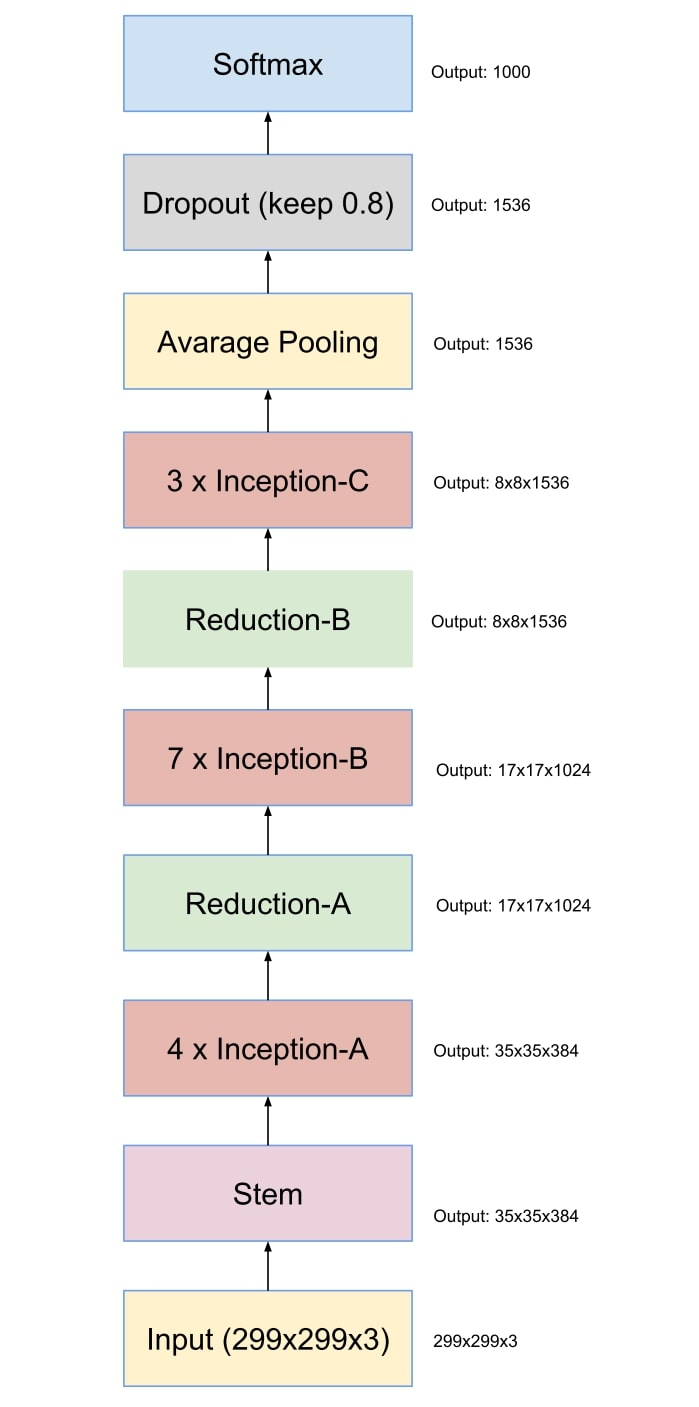
\includegraphics[scale=0.3]{inception_v4}
\caption{Inception-V4}
\label{fig:inception_v4}
\end{wrapfigure}

The contribution from Inception-V2 is batch normalization. They use ReLU as activation function in order to avoid the saturation problem and vanishing gradients. They had to use a higher learning rate for regularization because the output became more irregular. Last changes was reducing dimension by replacing   5×5 conv to two 3×3 convs. 

Inception-V4 also used the factorization from the Inception-V3. They reduce the dimensionality and it helped to decrease the overfitting problem. For example, if you have a 3×3 filter then you need 9 parameters, but the factorization idea proposes to operate  3×1 and  1×3 filters and use only 6 parameters. 

Inception-V4 have 3.1\% in Top-5 error rate and this result is better than winner of 2015 year ResNet (3.57\%) and  Inception-V3 (3.58\%). 

Inception architecture has a relatively low computation cost. Google try to make the inception module more efficient that's why they made it deeper and wider then Inception-V3 and they also simplify the architecture of this DNN.

Figure \ref{fig:inception_v4} shows the whole scheme for Inception-V4.

\subsection{GoogleNet}
GoogLeNet is a deep convolutional neural network and is also known as Inception-v1. The architecture based on \textit{Hebbian principle} with the intuition of multi-scale processing. Googlenet is 22 Layers deep network and used for object detection and classification. It has modules known as Inception which are a network within a network. GoogLeNet does not have any fully connected layers but uses global average pooling which keeps the model from overfitting the data.
It was able to achieve a top-5 error rate of 6.67\% and requires only 4 million parameters, whereas AlexNet requires up to 60 million parameters.

\subsubsection{Inception Module}
The logic behind Inception architecture is built on finding optimal local sparse structure in the convolution network and to repeat it spatially. There are 9 inception modules present in GooLeNet. Each Inception module has 6 convolution layers and 1 max pooling layer. Some Convolution layers and max pool layers are stacked on each other due to which four different outputs are created within the Inception module which are concatenated to produce one single output which is passed to next Inception module and so forth. Concatenation of this output filter occurs based on depth wise. The 1x1 convolution layers in Inception module help us to preserve spatial dimensions but to reduce the feature depth.

The output from the last Inception module is forwarded to global average pooling.

\begin{figure}[h!]
    \centering
    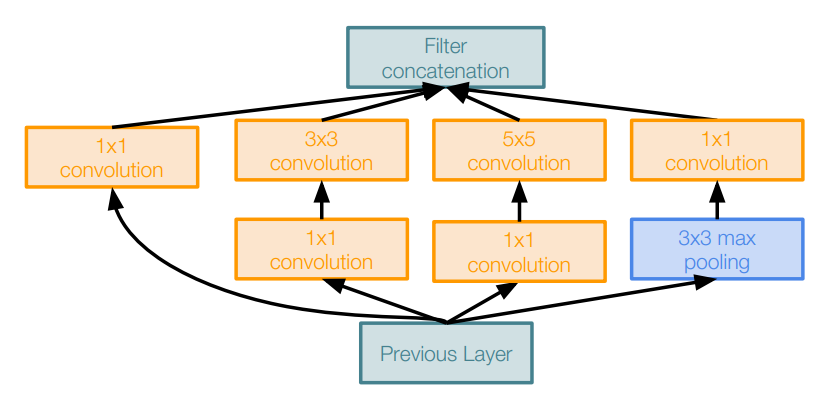
\includegraphics[scale=0.4]{googlenet}
    \caption{Inception Module}
\end{figure}

\subsection{Resnet50}
ResNet is another deep neural network released by Microsoft and, also, a winner of ILSVRG 2015 in image classification, detection, and localization. ResNet is a series of DNN with different numbers of layers from 18 to 152. The base idea is applying the residual connections which are described as learning the residual representation of functions instead of signal representation. One of the conceptual ideas of ResNet is using the skip connection. Skip connection makes the network deeper.  

Many convolution DNNs run into a problem with vanishing or exploding gradients because, during backpropagation, we derive error function with respect to the current weight and get multiplying of small or large numbers. The product of small numbers will be zero (vanished) and the product of large numbers will be too large (exploded). Developers of ResNet solved this problem by using a skip connection. In the skip connections for the next layer, they use the input from the previous layer without any modification. 

\begin{figure}[h!]
    \centering
    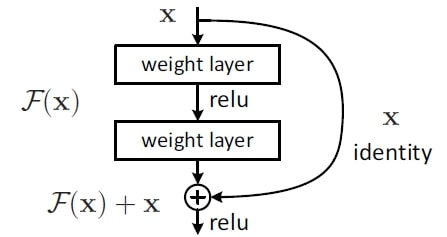
\includegraphics[scale=0.4]{resnet_1}
    \caption{Skip connection}
\end{figure}

\begin{wrapfigure}{l}{0.4\textwidth}
\centering
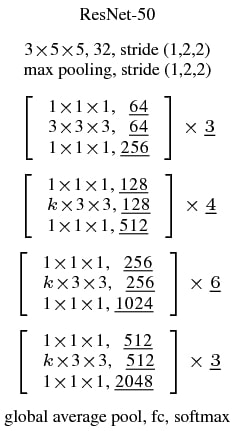
\includegraphics[scale=0.85]{resnet_2}
\caption{ResNet-50}
\label{fig:resnet_50}
\end{wrapfigure}

The output of skip connection is  F(x) + x and the weight layers actually are to learn a kind of residual mapping: output minus identity x. If we have a vanishing gradient we always have an identity x to send it back to previous layers. 

After each convolution layer ResNet use the batch normalization from Inception-V2. 

The main concepts of construction ResNet:
\begin{itemize}
\item avoiding representational bottlenecks by not abruptly reduce the dimension of data,but smoothly from the beginning of the network to the classifier at the output;
\item factorization of convolution layer into smaller pieces because this will save resources and help to increase the count of layers;
\item supporting a balance between the depth and width of the network. You should increase or decrease both dimensions.
\end{itemize}

Figure \ref{fig:resnet_50} shows the whole scheme for ResNet-50.
\pagebreak


\section{Datasets}
% Remove below lipsum command before posting your work
\lipsum[3]

\subsection{Imagenet}
% Remove below lipsum command before posting your work
It is one of the most prominent datasets used in the field of visual object recognition. In 2009 this dataset was first introduced to the world in the Conference on Computer Vision and Pattern Recognition by the computer science department from the Princeton University. It has over 14 million images and over 20000 categories. A large portion of the images have been hand annotated as well which can be helpful in the task of image captioning as well. Every year ImageNet runs a challenge called the ImageNet Large Scale Visual Recognition Challenge (ILSVRC), where different software architectures and algorithms take part in order to classify images of the dataset correctly. By 2017 most of the algorithms working on ImageNet have already achieved accuracy of more than 95%.

\subsection{CIFAR10}
% Remove below lipsum command before posting your work
Canadian Institute For Advanced Research is a widely used dataset in machine learning paradigm which is used in training various machine learning models. It is used in visual object recognition, It consist of 60000 images in total. The 10 stands for 10 classes in the dataset and each class has 6000 images which results into 60000 images of the dataset. Each image in the dataset is of 32*32 pixels coloured images. The 10 classes in the data set are air-planes, cars, birds, cats, deer, dogs, frogs, horses, ships, and trucks. Being only 32*32 pixel due to its low resolution it is one of the favourites for researchers to train their algorithms. 

\subsection{MNIST}
% Remove below lipsum command before posting your work
Modified National Institute of Standards and Technology is a database consisting of handwritten digits. This database is commonly used in the field of machine learning . It is a derived dataset from NSIT dataset. It consist of images which are 28*28 pixel size and greyscale nature. This dataset has been divided into 2 sets. To say in total in has 60000 training images and 10000 testing images. NSIT’s testing dataset contributes to one half of the training and testing database of the MNIST and the other half is filled by NSIT’s training dataset. The lowest possible error rate on MNIST achieved is 0.23% which was done by implementing a system of CNN’s.

\subsection{Selection of Dataset}
Reasons for selecting ImageNet
\begin{itemize}
    \item The MNIST and CIFAR 10 dataset are preliminary and intermediate dataset and does not pose a significant challenge in testing and training the complex CNN’s . also the topologies that are going to be used in the project are well optimised for a different dataset. Hence these are not being considered.
    \item On the other hand ImageNet provide a greater challenge and also the topologies that are going used have already used ImageNet dataset. Hence their result can be used as a benchmarking performance for the implementation in the project.
\end{itemize}

%End of the chapter



\chapter{Metrics}

\section{FLOPS}
Floating point operations per second (FLOPS) is a  unit of measure for the numerical computing performance of a computer. FLOPS is technically the right term to use when the data being worked upon is of floating point type.
In our case , with the quantization of weights from floating points  to integer type , we may have to refer to this unit of measurement as Integer Operations per Second (IOPS).
But the computing  industry and/or academia refers to ``just integer'' operations as MIPS (Millions of instructions per second). So depending on the eventual nature of the weights and the operational units on the FPGA,
we have to decide whether to report this performance measure in FLOPS or MIPS.  

To calculate FLOPS (and/or MIPS) , we look at the source code and the final profiler report from the executed code.
From the source code, we calculate the number of operations sans the overheads (loop index calculations, loop increment operations etc). And from the profiler report, we get a concrete idea of the clock frequency of the FPGA and the run time -– the execution time. Combining these two allows us to calculate  FLOPS/MIPS.


\section{Operations per cycle}
FLOPS/MIPS are quantities which are dependent on the clock frequencies supported by the FPGA boards.
When we want to just showcase the performance decoupled from the clock frequencies , we make use of Operations per cycle.
The way to measure Operations per cycle is similar to the way we find FLOPS. 

\section{Latency}
Latency is generally defined as the time delay between initial input to a system and the output from the system.
Latency captures the time it takes to load  data ,preprocess it, send said data over a network to the Inference Engine ,time needed for inference , and time needed to send the classified data back to the user.
Latencies can be measured for just a single image or over a batch of images. We can expect to have different latencies based on how we measure it(single image vs batch of images).

\section{Throughput}
Throughput is  a measure of amount of information processed per unit time. In our case , we define it as the number of bytes processed per second.
There are well known techniques to improve throughput like batch processing where a number of images is batched together and sent for inference job.
But as the batch size goes up , latencies also tend to go up. So there is a trade off involved here between through put and latency

\section{Accuracy}
Accuracy is defined as the fraction of the number of correct inferences made to the total number of inferences made.
In our context, accuracy depends on the CNN topology used , nature of weights , training data etc.


\section{Rate Correct Score}
Taking inspiration from the field of Memory and  Cognitive research , we can combine accuracy and latency by considering Rate Correct Score. It is defined as    

$RCS = \frac{c}{\sum R_t}$    

where   

$c$ = accuracy    

      $R_t$ = batch execution time  
      
Our aim would be to maximize RCS (either by increasng the accuracy or by decreasing the latency or both).


\chapter{Flowcharts}
% Remove below lipsum command before posting your work



\begin{figure}[h!]
    \centering
    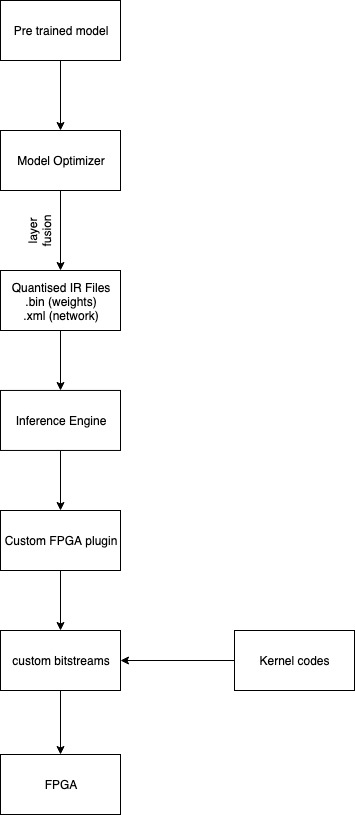
\includegraphics[scale=0.65]{open_vino_flowchart.jpg}
    \caption{Open Vino Flowchart}
\end{figure}


%End of the chapter

\chapter{Technologies}

\section{OpenVINO}
% Remove below lipsum command before posting your work
Intel OPENVINO is an open source toolkit from Intel that allows the deployment of pre-trained deep neural networks on different hardware platforms such as CPU, GPU, FPGA etc. The toolkit is available for installation for the Windows operating system as well as selected Linux distributions. All of the tool's libraries and plugins except the FPGA plugin are a part of the open source github repository.
The functionality of OPENVINO is divided among its components, Model Optimizer, Calibration Tool,  Inference Engine. This is shown in Fig 5.1 and explained below. 

\subsection{Model Optimizer}
The Model Optimizer is a python based tool which takes as input a pre-trained model. It supports many popular deep learning frameworks such as TensorFlow, Caffe, PyTorch, MXnet etc. This model is then converted to a common intermediate format (IR), thereby making the inference engine independent of the training framework. The IR contains a .xml file which represents the computational graph of the CNN and a .bin file containing the weights. The graph is optimized by fusing different layers of the original topology wherever possible. The weights are accordingly adjusted. The toolkit comes with a model downloader which can download various openly available pre-trained models for different frameworks.
 
\subsection{Calibration Tool}
 The Calibration Tool, added in the recent release of the toolkit, performs post training quantization to int8 before the IR is passed on to the inference engine.  The tool is open source. 
 
 \subsection{Inference Engine}
 The Inference Engine is responsible for the execution of the model on the selected hardware. For this purpose, it provides a C++ API which can be integrated in an application. The main task performed by the inference engine is to read the Intermediate Representation of the model, select the hardware for deployment such as CPU or FPGA and call the appropriate plugin which defines all necessary data structures and functions required to perform inference and return the output along with performance statistics. 
 The toolkit comes with pre-compiled bitstreams (.aocx files) for a few supported FPGA boards. These bitstreams implement various popular network topologies such as GoogleNet, ResNet etc. as well as generic layers which are used to program the FPGAs as per the requirement of the given model topology. 
 \subsection{Advantages}
  
 \begin{itemize}
 \item Supports optimization of models and quantization of weights.
 \item A CNN model can be deployed on hardware with minimal programming effort and independent of the training framework.
 \item For FPGAs, the use of pre-compiled bitstreams eliminate the time needed for synthesis of kernel codes.
 \end{itemize}
 
 \subsection{Disadvantages}
 \begin{itemize}
 \item The main disadvantage is the compatibility of FPGA boards. Development and synthesis of kernel codes along with a plugin for FPGAs may be required to make OPENVINO work with unsupported boards. 
 \item Scaling to multiple FPGAs, which is one of the goals of this project is non-trivial as it would require development of overlays for external I/O channels. 
 \end{itemize}
\section{TVM}

Today we have a lot of different deep learning frameworks such as TensorFlow, Cafee2, MXNet and PyTorch and hardware targets: CPUs, GPUs, FPGAs, and ASICs. During the mapping of one of the frameworks to a device, we run into the problem with a variety of hardware characteristics such as memory organization (implicitly managed, mixed, explicitly managed) and compute primitives (scalar, vector, tensor).

TVM takes the model from different learning frameworks and generates optimized code for devices. TVM was started as a research project at the Paul G. Allen School of Computer Science & Engineering, University of Washington.

TVM includes a computational graph rewriter, tensor expression language and new features for GPU accelerators.

The system has the stack of implementation: NNVM $\to$ TOPI $\to$ TVM $\to$ VTA. NNVM acts as a graph optimizer by taking the model from an existing framework  and converting it into “TVM” graph. For these operations, we use the TOPI language. TOPI is a library where functions operate as instructions for further work. For example, TOPI defines a tensor computation, schedules space for each NN operator (e.g. conv2d). The next step is the application of the TVM functions. TVM uses the TOPI instructions and generates code for several backends, such as LLVM, or CUDA etc. The final step is the Versatile Tensor Accelerator (VTA) which is responsible for the stream and microkernels. 

In order to change a hardware target ( CPU, GPU or TPU) we need to rebuild TVM libraries again.  

\begin{figure}[h!]
    \centering
    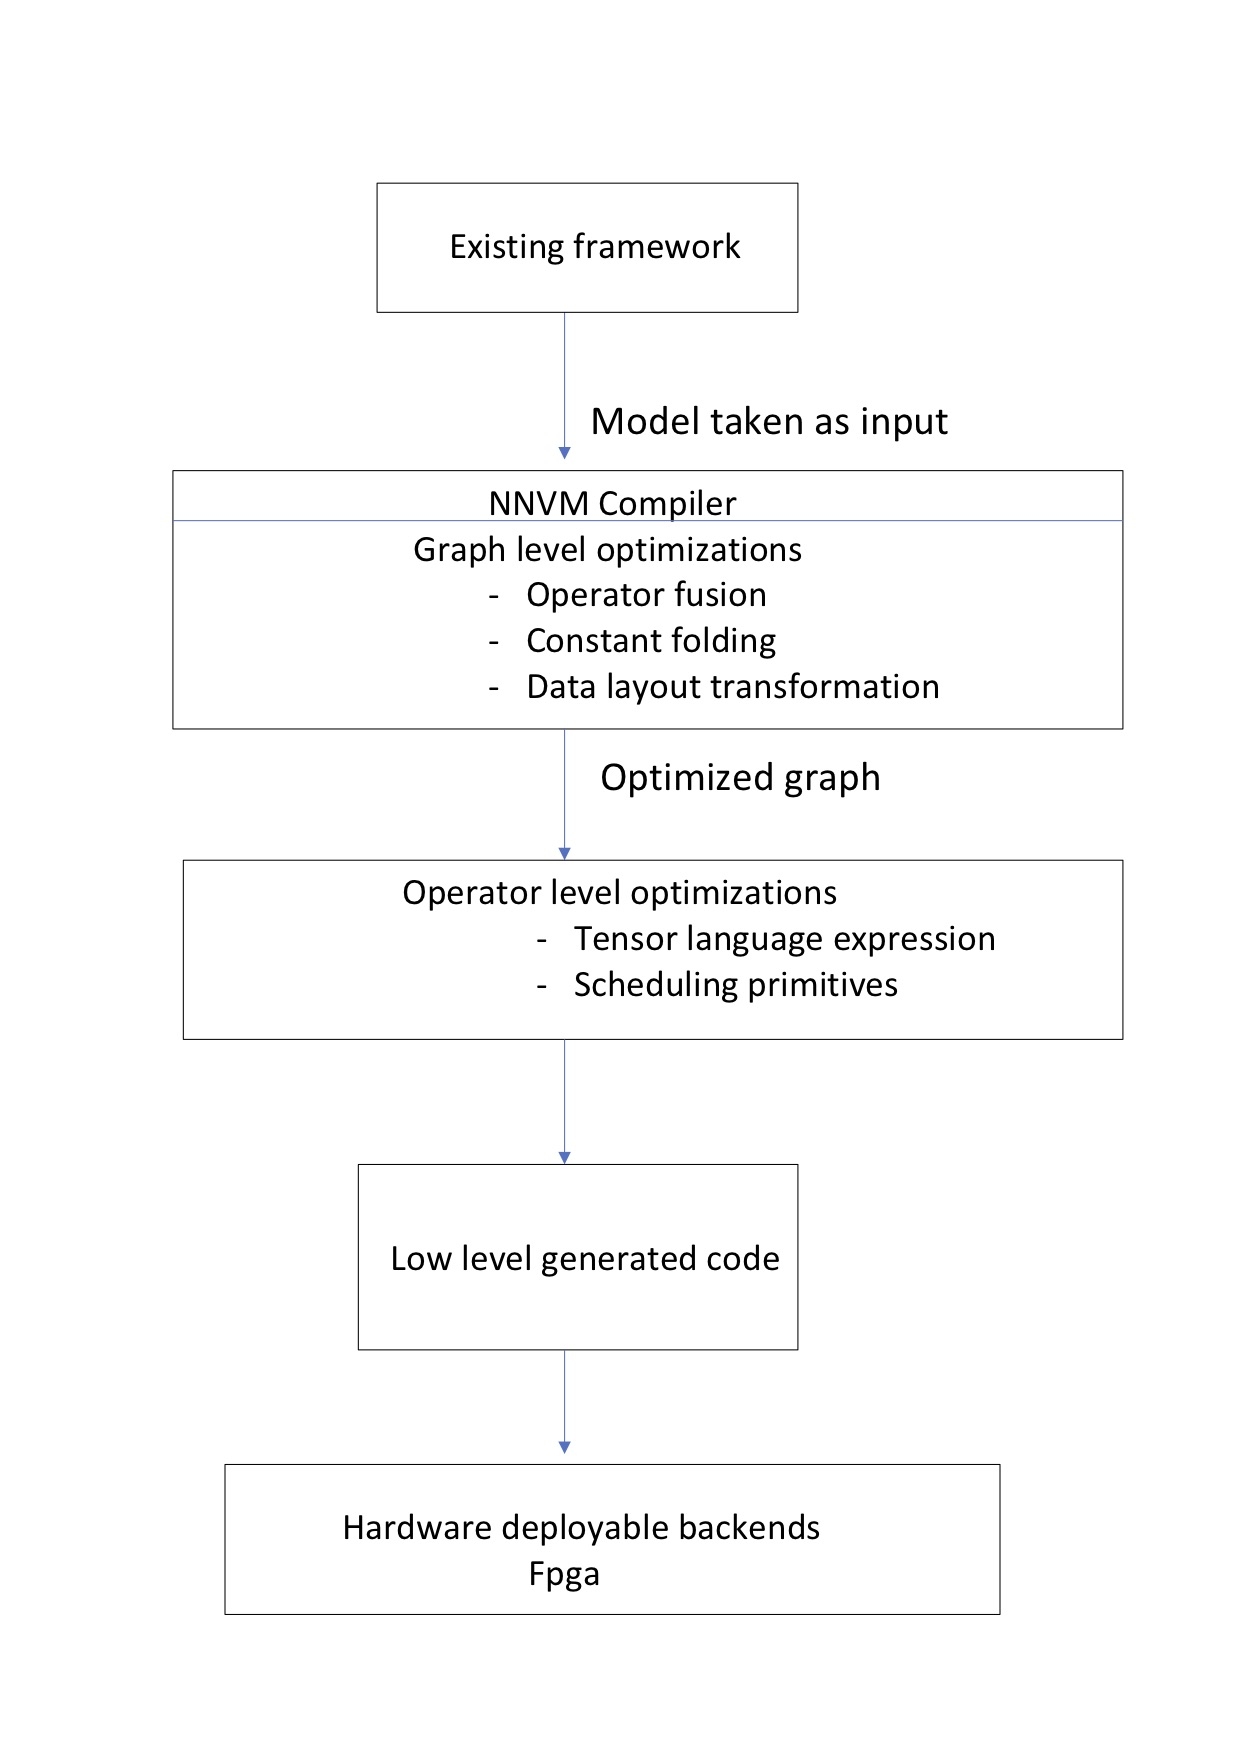
\includegraphics[scale=0.19]{TVM_Flowchart.jpg}
    \caption{TVM Flowchart}
\end{figure}
 
 \subsection{Advantages}
 \begin{itemize}
 \item TVM is a open-source product;
 \item TVM supports AOCL backend, but this option is still experimental. Information was updated in October 2018;
  \item It is planned to implement a different quantization schemes (Symmetric, Asymmetric, Channel-wise Scale) for different bits (i8 $\to$ i32, i16 $\to$ i32, i8 $\to$ i24, i5 $\to$ i16);
 \end{itemize}

 \subsection{Disadvantages}
 \begin{itemize}
 \item There is no information about which FPGA boards are supported by TVM.
 \end{itemize}

\section{Xilinx}
Xilinx Machine Learning Suite toolchain provides us tools to develop and deploy machine Learning applications in Real-time Inference. It provides machine learning inference with low-latency and high throughput. The suite also provides support for widely used machine learning frameworks such as Caffe, Tensorflow, MXNet.

The functionality of ML-Suite is divided among its components: Machine Learning Framework, xfDNN Middleware, and xDNN IP.

\subsection{Machine Learning Framework}
Xilinx ML Suite supports various frameworks such as Caffe, Tensorflow, Keras, MXNet, Darknet. Support for various other frameworks can also be provided with help of \textit{Open Neural Network Exchange} (ONNX).

\subsection{xfDNN Middleware}
It is a high-performance software library and provides API which works as a bridge between xDNN IP which runs on FPGAs and ML frameworks such as Caffe, Tensorflow. xfDNN requires SDAccel reconfigurable acceleration environment for running it on Xilinx FPGAs and currently is the only middleware available for programming ML frameworks on Xilinx FPGAs. xfDNN middleware has the following components:
\subsubsection{Compiler}

It provides tools for network optimization such as layer fusions, memory dependency optimization, removing CPU host control bottlenecks with network pre-scheduling. It creates a "one-shot" execution flow for the network to run on FPGA.

\subsubsection{xfDNN Quantizer} 

xfDNN Quantizer enables fast, high-precision calibration to lower precision deployments to INT8 and INT16. It performs a quantization technique known as a recalibration.

\subsection{xDNN IP}
Xilinx xDNN IP cores are high-performance general CNN processing engines. Various different types of CNN networks and models can be executed on these engines. They have two DSP Array configurations available (28x32 and 56x32). 28x32 configuration provides higher throughput whereas 56x32 can fit larger models at low latency.
xDNN provides Overlay to combine various xDNN IP kernels.

\subsection{Advantages and Disadvantages}
  
 \begin{itemize}
 \item Supports model optimization and weights quantization.
 \item Delivers high throughput and low latency.
 \item Compiler and Quantizer can be used separately and does not require a Xilinx environment.
 \item Does not support fully connected and softmax layers.
 
 \end{itemize}



%End of the chapter

\chapter{Related Work}
% Remove below lipsum command before posting your work
\textbf{[1]Deep Neural Network Approximation for Custom Hardware: Where We've Been, Where We're Going}

We know that FPGA's and ASIC's increase the speed of inference, while GPU still excel at floating point operations. The need of the hour is to have high throughput and high efficiency which can be achieved with the help of custom hardware and low precision quantization. Hence a lot of research and work is going on in the field of DNN approximation techniques based for custom hardware. One of the most prominent and ongoing research field in the approximation of DNN is the technique of quantization. Jacob et al. used 8-bit quantization in implementation of MobileNet CNN which saw 50 percent
 decrease in inference latency. From there on several papers have been published which show implementation of various quantization techniques and their effects on throughput and how they were able to achieve various compression ratio factors but along with that there were accuracy loss that incurred at the cost of quantization. To cite a few Courbariaux et al, Qiu et al. and Shin et al.(2015) implemented block floating point and there CNN gave a 1.0 pp accuracy loss. Jing Li et al, proposed Adaptive quantization in (2018), Do-Re-Fa Net uses a very similar approach as to the one proposed by Jing Li et al. Ma.hieu Courbariaux and Yoshua Bengio.  Proposed binarization technique in Binary Connect, which was able to achieve less than 1 pp accuracy losses(2016). Similarly other techniques like ternarization , Fine grained quantization and Logarithmic quantization were also implemented and these techniques showed better performance than the standard CNN which used FP32 bit representation. 

\textbf{[2]Toolflows for Mapping Convolutional Neural Networks on FPGA's : A Survey and Future Directions}

In this paper, the authors have presented a survey on the existing CNN-to-FPGA tool-flows which are
evaluated on the basis of different parameters and performance metrics. This paper also gives an insight
on different Design and Space Exploration Strategies and architectural decisions. At last all of the
discussed tool-flows are tested against state-of-the art Neural Network models such as GoogleNet ,
VGG16, ResNet-152 etc.
One of the key sections of the survey was about the architecture that each of the tool-flows adhere to.
There are two types:
\begin{itemize}
\item Streaming Architecture : In this type of architecture we assign a hardware block to each layer. These
layers are chained to form a pipeline. Using this principle we will be implementing the streaming
architecture in our project. This type of architecture favors optimization
\item Single Computation Engine: This architecture is used to form an overlay. This provides flexibility,
portability, fast configuration time. This architecture is independent of the host FPGA. Scheduling is done
under the hood. Customization of the network can be a challenge here.
\end{itemize}


%End of the chapter

\chapter{Time plan}
In this section we describe how we plan to plan and monitor our project. Since the tutorial phase and research phase were well managed and organized by our mentor Tobias, the scope of this section is limited to second phase of the project. This section is divided into several parts and each part explains project’s organizational decisions. 

\section{Project Meetings}
% Remove below lipsum command before posting your work
: Project meetings will be held twice in a week. Currently it is being held on Mondays (1pm to 4pm) and Wednesdays (9am to 12pm). In these meetings, all the project members gather and discuss the current updates in the project. It covers mainly three things. Firstly, the general project updates. Secondly individual task updates where each participant updates about his/her work to the team. Lastly, the issues being faced. 
After each meeting, the minutes of the meeting will be prepared by one of the team member’s. The assignment of this task is based on round robin fashion. All MoMs will be uploaded to project’s Git repository.


\section{Project Phases}
\subsection{Project Planning}
% Remove below lipsum command before posting your work
In this phase, we decide on the goals, feasibilities of achieving these goals, prioritizing and the overall organization of the project which will be followed till the completion of the project. This involves defining the scope, dividing the project into subgroups, assigning roles and responsibilities (such as project lead, Git master). Here we define the phases and also estimate the time required. 

\subsection{Finalizing the Plan and Mini Presentation}
% Remove below lipsum command before posting your work
During this phase, we finalize the tools, organizations and present a talk on how our final project will look like using a PowerPoint presentation or a diagram on board. It will be a simple visualization of the entire idea. This will portray a clear picture before the mentor and the team members before going to the upcoming phases which highly depend on this plan. Outcome of this phase will be a final Project Plan document reviewed by Tobias. 

\subsection{Design}
The whole architecture of the project will be designed via a Flow chart. Before we start to implement, this will show us HOW we will achieve the goals defined earlier. Outcome of this phase will be a final design document. 

\subsection{Implementation and Testing}
The most important phase of our project is this phase and arguably the lengthiest phase. We assume the best case scenario that all our requirements are fixed but in case of additional requirement or change in requirement, we will meet and discuss to accommodate them. 

In this phase we start coding by keeping the goals in mind and start implementing the tasks assigned to us. This phase will also include testing and fixing bugs therefore coding and testing will go hand in hand. At the end of this phase, we will have a working application that meets the goals we defined. 

\subsection{Result collection and Performance Evaluation}
Since one of main goals of the project is performance optimization, we will run the application to collect the result. After collecting, we will look into whether we are doing best in terms of first – our set goals, secondly – results in comparison with state of the art benchmarks. If we find deviation or find there is a room for improvement, we go back to the previous phase.

\subsection{Final project report and Presentation}
After achieving the desired results, we will prepare a final project report that covers all the aspects of our project in detail. At the end, we will present the implementation via a demo and show experimental results. 

The Below picture shows the time plan for each phases. Some of these phases will overlap based on dependability.

\begin{table}[]
\begin{tabular}{|l|l|l|l|l|l|l|l|l|l|l|l|l|l|}
\hline
                                             & \multicolumn{13}{c|}{TIME}                                                                                                                                             \\ \hline
Project Phases                               & \multicolumn{2}{l|}{Mar} & \multicolumn{2}{l|}{Apr} & \multicolumn{2}{l|}{May} & \multicolumn{2}{l|}{Jun} & \multicolumn{2}{l|}{July} & \multicolumn{2}{l|}{Aug} & Sep \\ \hline
Project Planning                             &            & x           &             &            &             &            &             &            &             &             &             &            &     \\ \hline
Finalizing the plan and mini-presentation    &            & x           & x           &            &             &            &             &            &             &             &             &            &     \\ \hline
Design Phase                                 &            &             & x           & x          &             &            &             &            &             &             &             &            &     \\ \hline
Implementation and Testing                   &            &             &             & x          & x           & x          & x           & x          &             &             &             &            &     \\ \hline
Result collection and Performance Evaluation &            &             &             &            &             &            & x           & x          & x           & x           &             &            &     \\ \hline
Final Project Report and Presentation        &            &             &             &            &             &            &             &            &             & x           & x           & x          & x   \\ \hline
\end{tabular}
\end{table}
%End of the chapter

\chapter{Conclusion}

% Remove below lipsum command before posting your work
To recap the project plan, we are trying to build a system which performs as good as or better than State of the art inference systems by leveraging the infrastructure available in PC2. Currently we have finalized on the Datatset we are going to use(ImageNet), and the CNN Topology (GoogleNet, Inception V4 and Resnet52). The next challenge is to divide the work of developing a plugin for Intel OpenVINO and meanwhile implement a simple model in TVM. For the future phase, We will use TVM to generate OpenCL kernels on our model. Later, we will transfer these decisions to a small talk before the research group before starting the project.

%End of the chapter

\end{document}
